\chapter{Literature Review}
	\section{Chapter Overview}
		This chapter details the background research that was carried out in order to make informed decisions during the project. 
	\section{Natural Language Processing}
		\subsection{Evaluation of Binary Classification Algorithms}
			A binary classification model is an algorithm that sorts a set into two categories. One set is often referred to as 'positive' and the other 'negative'. It is important to validate a model in order to see whether its results can be trusted. Upon validating, if an item in the set has been correctly classified, it is considered a 'true' classification, otherwise, it is considered a 'false' classification. 

			The holdout method of validation involves training the model on a large proportion of the data, known as training data, and then classifying the rest of the data, known as test data, and giving the model a score based on how the test data was classified based on their actual class. This is limited as the test data set may be overfit to the model, making the model perform better for that test data than it would for new incoming data. Two common methods of solving this problem are cross-validation and bootstrapping.  

			Cross-validation is where the dataset is split into $k$ segments. Each segment is treated a training data $k-1$ times and treated as test data once. This will give $k$ different scores for the model. Meanwhile, bootstrapping is where $n$ items in the dataset are picked uniformly at random. Each item is put back into the dataset once picked. This can be done several times to produce different scores for the model. In both cases, if the scores have a high average and low variance, the model is successful and not overfit to the data. 

			Kohavi compares these methods and recommends the use of cross-validation because bootstrap can be prone to large biases\cite{cv_bootstrap_kohavi}. Kohavi found that the optimum number of folds depends on the stability of the dataset. He also notes that cross-validation's evaluation is most accurate when each fold is stratified to have a similar number of each class in it. 

			The simplest score that can be used for a model is accuracy. Accuracy is the ratio of correctly classified test documents to the total number of test documents. This is insufficient for imbalanced datasets\cite{balanced_accuracy_velez}.
			
			A common solution to this in topic classification is to use precision, which is the ratio of true positives to the total number of positive classifications shown in Equation \ref{equ:precision}, and recall, which is the ratio of true positives to the total number of classifications made in total, shown in Equation \ref{equ:recall}. Precision and recall can be combined in two ways. The F1 score finds the harmonious mean between the two as shown in Equation \ref{equ:f1}. The precision/recall breakeven point is obtained by modifying the classifying threshold until the precision and recall values are equal\cite{ml_automated_sebastiani}. These methods are most appropriate for information retrieval when it is important to evaluate true positives and true negatives are in excess\cite{markedness_correlation_powers}.
			\begin{equation}\label{equ:precision}
				precision = \frac{tp}{tp + fp}
			\end{equation}
			\begin{equation}\label{equ:recall}
				recall = \frac{tp}{tp + fn}
			\end{equation}
			\begin{equation}\label{equ:tnr}
				tnr = \frac{tn}{tn + fp}
			\end{equation}

			Velez suggests balanced accuracy, shown in Equation \ref{equ:bacc}, as the solution. This is the average of the true positive rate, which is another name for recall shown in Equation \ref{equ:recall}, and the true negative rate, which is the ratio of true negatives to the total number of classifications made shown in Equation \ref{equ:tnr}. This method is more appropriate for cases where it is important to evaluate both the true positives and the true negatives.

			\begin{equation}\label{equ:f1}
				f_1 = 2 \times \frac{precision \cdot recall}{precision + recall}
			\end{equation}
			\begin{equation}\label{equ:bep}
				BEP = precision = recall
			\end{equation}
			\begin{equation}\label{equ:bacc}
				balanced\textnormal{-}accuracy = \frac{recall + tnr}{2}
			\end{equation}

			Tables \ref{tab:unbal-neg} and \ref{tab:unbal-pos} show how the different scoring systems rate the performance of imbalanced datasets and algorithms. The algorithms both classify a given test item into a predetermined class, regardless of the item's contents. Balanced accuracy is the only scoring system to rank both algorithms poorly.
			
			\begin{table}
				\parbox{.45\linewidth}{
					\centering
					\begin{tabular}{l|c}
						\hline
						type&score\\
						\hline
						accuracy&0.95\\
						$f_1$ score&0\\
						BEP&0\\
						BACC&0.48
					\end{tabular}
					\caption{Scores with a ground truth of 5 positives and 95 negatives and a prediction of 0 positives and 100 negatives.}\label{tab:unbal-neg}
				}
				\hfill
				\parbox{.45\linewidth}{
					\centering
					\begin{tabular}{l|c}
						\hline
						type&score\\
						\hline
						accuracy&0.95\\
						$f_1$ score&0.97\\
						BEP&0.95\\
						BACC&0.48
					\end{tabular}
					\caption{Scores with a ground truth of 95 positives and 5 negatives and a prediction of 100 positives and 0 negatives.}\label{tab:unbal-pos}
				}
			\end{table}
		\subsection{Topic Classification}\label{ssec:topclas}
			Document topic classification is the automated assignment of natural language texts to predefined categories based on their content\cite{ml_automated_sebastiani}.  

			Support vector machines are a common feature-based approach to classification. They work by considering features, which are to be discussed in Section \ref{litrev-langfet}, and plotting each document in the feature space by the number of times each feature occurs in it. It then plots a hyperplane that best splits each document class, as exemplified by Figure \ref{fig:svm_simple}. This led to an 0.86 precision/recall breakeven point when Joachims classified the Reuters 'acq' dataset\cite{svm_joachims}.  

		\begin{figure}[h]
    		\centering
    		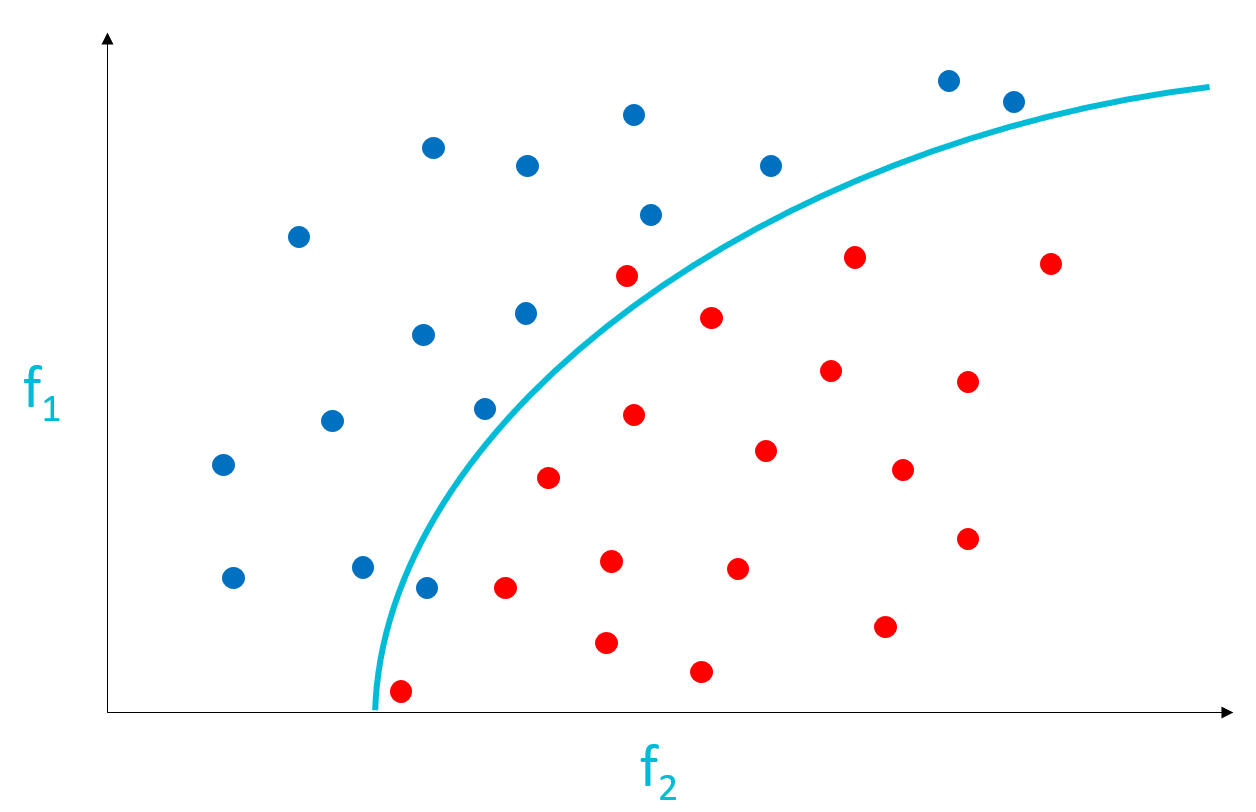
\includegraphics[width=0.5\linewidth]{resources/images/svm_simple.png}
    		\caption{A simplified example of how Support Vector Machines work.}
    		\label{fig:svm_simple}
		\end{figure} 

			In contrast, Naive Bayes is a probabilistic approach based on Bayes' rule. Bayes' rule, shown in Equation \ref{equ:nb}, is a formula for finding the probability of class $C_k$, given a set of features $x$. There are many variations of this type of classification where the likelihood, representing the probability of a document given a class, differs. The Bernoulli multivariate model only considers whether a word occurs in a document while the multinomial model considers how many times a word appears in each document. Predictably, McCallum and Nigam found that the multinomial model performs consistently stronger over any significant vocabulary size. This led to a 0.89 precision/recall breakeven point when classifying the Reuters 'acq' dataset, slightly better than Support Vector Machines 0.86.  

			\begin{equation}\label{equ:nb}
				p(C_k|\textbf{x}) = \frac{p(C_k)p(\textbf{x}|C_k)}{p(\textbf{x})}
			\end{equation}

			Wang and Manning improved the performance of both naive Bayes and support vector machines, for datasets with average wordcounts over 100, by adding elements of naive Bayes to support vector machines\cite{baselines_bigrams_wang}.  

			All these methods assume that each document can only be a member of one class. This is often not the case. Godbole and Sarawagi use the example that if a document is classed as being about wheat, it is also likely to be about grain\cite{discriminative_multilabel_godbole}. This relationship between topics can be captured in a topic-topic distribution and used to enhance results. Godbole and Sarawagi implement a few variations of this, all based around the standard support vector machines with one added feature per class representing how similar the given class is to all other classes. It leads to a slight improvement of F1-score across two datasets.
			
			% Neural network topic classification
		\subsection{Sentiment Analysis}
			The same classification techniques used in topic classification in Section \ref{ssec:topclas} can be used for sentiment analysis as demonstrated by Moraes et al who experimented with SVM, naive Bayes and artificial neural networks. They classified reviews as positive or negative with a 0.87 accuracy score using neural networks on a movie reviews dataset\cite{sentiment_ann_moares}. Using these machine learning techniques, however, needs significant data to train on which is not always available. 
			
			An alternative method for sentiment analysis is a lexicon based approach. As a preliminary investigation, Pang et al obtained a list of positive keywords and a list of negative keywords for a different set through analysis of the term frequencies of a set of training data\cite{sentiment_ml_pang}. They then classified the test data based on whether they had more positive or negative keywords. This achieved an accuracy of 0.64, performing significantly worse than Moares et al at the same task.
			
			Mandal and Gupta propose a more advanced lexicon based approach\cite{lexicon_sentiments_mandal}. This involves a detecting comparative and superlative words and assigning a higher weighting when these precede a keyword. Most notably, it involves negating rating should negation words such as 'not' appear before a keyword. This increased Mandal and Gupta's accuracy from 0.87 to 0.97 on their manually created online review dataset.			
		\subsection{Language Features}\label{litrev-langfet}
			In natural language processing, each document is represented as a set of features where each feature is given a value. The simplest set of features a document can have is the set of unique words that appear in the document. This is known as the bag of words model. It has the benefit of having dense feature spaces, meaning that there is a low number of features which reoccur many times in the document. Dense feature spaces are more computationally efficient than sparse feature spaces. However, bag of words is limited in that these features are less capable of conveying the document's meaning. For example, Wallach points out that the phrase “the department chair couches offers” has a different topic to “the chair department offers couches”, yet a bag of words model will represent them as the same\cite{beyond_bag_wallach}. This sort of ambiguity would clearly give inaccurate results so it is worth using a feature a bit more resource heavy that provides more accuracy.  

			The most common feature used is an n-gram model. This is where $n$ words are taken as the feature, giving each feature context. For example, a 5-gram would have the capability to distinguish between the above examples. However, the higher n is the less computationally efficient the processing will be and Tan et al found that the pay-off in computational efficiency was not worth it for n=3 but was for n=2\cite{bigrams_enhance_tan}. There are methods to improve computational efficiency, such as filtering out all features that do not meet some threshold. Tan et al's found that filtering out all features that appeared in less than three documents or less than 0.5\% of documents helped sufficiently. Implementing bigrams and combining them with the documents' unigrams, resulted in an average F1-score improvement of 0.03 on the Reuters datasets\cite{bigrams_enhance_tan}. 

			Alongside changing the type of features, the way that features are counted can be changed. The simplest form of this is counting the features as binary, representing a feature as 1 if it occurs in a document and 0 if it does not. Another simple count is to represent a feature by the number of times it occurs in a document. This method gives more influence to longer documents. Term frequency, shown in Equation \ref{equ:tf}, solves this by dividing the term count by the total number of words in the document. Inverse document frequency, shown in Equation \ref{equ:idf}, gives a higher weight to words that appear in low amounts of words. Term frequency-inverse document frequency (tf-idf) is a combination of its namesake methods, shown in Equation \ref{equ:tfidf}. Lan et al investigate these methods and variants of them and find that term frequency performs better than tf-idf frequency for the Reuters dataset despite tf-idf being the standard.
			
			\begin{equation}\label{equ:tf}
				tf = \frac{f_{t,d}}{\sum_{t' \in d}f_{t',d}} 
			\end{equation}
			\begin{equation}\label{equ:idf}
				idf = \log \frac{N}{n_j}
			\end{equation}
			\begin{equation}\label{equ:tfidf}
				tf\textnormal{-}idf = tf * idf
			\end{equation}
			
			Liu and Yang proposed a simple improvement to tf-idf named term frequency-inverse document frequency-class frequency (tf-idf-cf), shown in Equation \ref{equ:tfidfcf}\cite{tfidfcf_categorization_liu}. This adds weight to a term if it commonly occurs in the document's class. This gave a 0.08 accuracy improvement over tf-idf on the Reuters dataset.
			\begin{equation}\label{equ:tfidfcf}
				tf\textnormal{-}idf\textnormal{-}cf = tfidf * \frac{n_{cij}}{N_{ci}}
			\end{equation}
		\subsection{Detecting Trends}
			Regression analysis is the construction of mathematical models which explain relationships between variables. Ordinary least squares is the simplest regression technique intuitively. A line $f(x,\mathbf{\beta})$ is constructed from the parameters $\mathbf{beta}$ that minimise the total squared distance, $S(\mathbf{\beta})$, of the line to each predicted input $y_i$\cite{regression_analysis_seber}. 
			
			\begin{equation}\label{equ:param}
				f(x,\mathbf{\beta}) = \sum \beta_j \phi_j(x)
			\end{equation}
			
			\begin{equation}\label{equ:regdistance}
				r_i(\mathbf{\beta}) = y_i - f(x_i,\mathbf{\beta_i})
			\end{equation}
			
			\begin{equation}\label{equ:regsum}
				S(\mathbf{\beta}) = \sum r^2_i(\mathbf{\beta})
			\end{equation}

			The least squares method can produce lines that are not straight using polynomial linear regression where $\mathbf{\beta}$ remains linear but the $x$ inputs are polynomials. Alternatively, a nonlinear method can be used which involves the $\mathbf{\beta}$ parameters taking the form of functions\cite{nonlinear_regression_motulsky}.
			
			Ordinary least squares works on the assumption that all distances are errors that are independent and identically distributed normally. However, a single grossly out-lying observation can spoil the estimate\cite{robust_regression_huber}. The solution to this is to modify least squares in order to make the estimate less sensitive to extreme values of residuals. This is called robust regression.				\subsection{Statistical Significance}
			If a linear regression line has a gradient not equal to zero, there is a relationship between the variables. It is very likely that this will be the case but it is not necessarily the case that the gradient will be similar every time. Statistical significance is the idea that a claimed trend has not happened by chance and will consistently occur with other data. Fisher arbitrarily dictated that a trend is statistically significant if its p-value is less than 0.05\cite{stats_research_fisher}.
			
			A p-value is the probability that a statistical summary of the data would be equal to or more extreme than its observed value\cite{statement_p_wasserstein}. It is worked out based on the gradient's t-value. A t-value is the ratio of the difference between the estimated value of a parameter, from its hypothesised value and the standard error. For finding the statistical significance of a gradient, the estimated value of the parameter, is the gradient worked out in linear regression and the hypothesised value is zero.  

			However, the importance of p-values has come into question since many scientific claims have turned out to be false despite being backed by p-values. Benjamin et al recommend reducing the statistical significance threshold to 0.005 to ensure it is very likely to be statistically significant before making any bold claims\cite{redefine_statsig_benjamin}. The American Statistical Association, meanwhile, just warn that statistical significance should not be taken as gospel and any decisions came to based on p-values should be assisted by thorough human analysis\cite{statement_p_wasserstein}. As well as this, Boos and Stefanski question the reproducibility of p-values and encourage cross-validation-like methods to ensure that a claim is statistically significant\cite{p_reproducibility_boos}. 
		\subsection{Pre-processing}
			Pre-processing text before classification is where text is formatted and changed before classification. It primarily reduces the feature set which improves the efficiency of classification but it can also improve classification accuracy. Three of the main pre-processing methods are stemming, removing stopwords, lowercasing.
			
			Stemming is where the suffix of a word is removed in order to collate all variants of the same word. This would change the words 'property' and 'properties' to 'properti'. Lemmatising is a similar method performing same the task which removes the suffix of a word but then replaces it with a standard suffix so it is still a valid word\cite{influence_normalization_toman}. This would change both 'property' and 'properties' to 'property'. Toman et al found that both stemming and lemmatising either made no significant improvement on classification or gave significantly worse classification results than using neither method\cite{influence_normalization_toman}. Meanwhile, Uysal and Gunal found that whether there was performance improvement with stemming was dependent on the domain but the proportion of words that were stemmed were up to 0.45\cite{impact_preprocessing_uysal}, therefore, increasing the efficiency of the classification.
			
			Stopwords are words that are so common in all classes that they make no difference to classification and therefore, there may be no point in including them. This includes words such as 'the', 'and' and 'i'. Interestingly, Toman et al found that stopwords should be taken out of text as that improves classification but Uysal and Gunal found that stopwords should be left in as they can inadvertently indicate class. This reaffirms Uysal and Gunal's hypothesis that there is no set of pre-processing methods that can be applied to all domains and they should instead be experimented with.
			
			Lowercasing is replacing all capital letters with lowercase letters so a normal word is treated as the same word even when it is at the start of the sentence. Uysal and Gunal found this made a significant improvement to classification in all domains.
	\section{Visualisation}
		\subsection{Displaying Trends}
			Gestalt set out principles of visual perception. These are widely used in information visualisation because they aid understanding of how people perceive patterns\cite{gestalt_graph_kobourov}. The following list is a subset of Gestalt principles that are most useful for emphasising trends and anomalies:
			
			\begin{itemize}
				\item Proximity, illustrated in Figure \ref{fig:proximity}, is the idea that groups of objects that are close together are quickly identified as a group;
				\item Similarity, illustrated in Figure \ref{fig:similarity}, is the idea that objects that have similar attributes, such as colour or shape, are quickly identified as a group;
				\item Enclosure, illustrated in Figure \ref{fig:enclosure}, is the idea that objects that are encapsulated by another object are quickly identified as a group;
				\item Figure \& ground, illustrated in Figure \ref{fig:figure_ground}, is the idea that a perceived foreground and background are quickly identified as two separate groups. 
			\end{itemize}
			
			\begin{figure}[!htb]
				\minipage{0.23\textwidth}
  					
\includegraphics[width=\linewidth]{resources/images/proximity.png}
  					\caption{An illustration of proximity.}\label{fig:proximity}
  				\endminipage\hfill
  				\minipage{0.23\textwidth}
  					
\includegraphics[width=\linewidth]{resources/images/similarity.png}
  					\caption{An illustration of similarity.}\label{fig:similarity}
  				\endminipage\hfill
  				\minipage{0.23\textwidth}
  					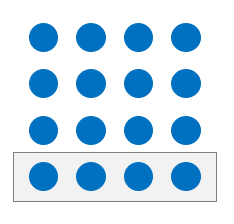
\includegraphics[width=\linewidth]{resources/images/enclosure.png}
  					\caption{An illustration of enclosure.}\label{fig:enclosure}
  				\endminipage\hfill
   				\minipage{0.23\textwidth}
  					
\includegraphics[width=0.75\linewidth]{resources/images/figure_ground.png}
  					\caption{An illustration of figure \& ground.}\label{fig:figure_ground}
  				\endminipage\hfill
			\end{figure}
			
			Healey extends upon this by investigating preattentive features of objects\cite{attention_visualizaton_healey}. Preattentive features are features which are identified immediately as an image is first scanned. These included length, width, volume, orientation, number, density, curvature, closure, terminators, colour, luminance and more. The idea is that a human can identify any inconsistencies in these features without having to think, such as if there is one red dot among many blue dots. It is important to note that some features are assymetric, for example, a curved line among vertical lines can be identified preattentively but a vertical line among curved lines cannot be. Healey also investigated how visual features compete for attention. The purpose of this is so the most important information can be encoded to be processed earliest. He identified the order of processing of visual features as follows:
			
			\begin{enumerate}
				\item Determine the 3D layout of a scene;
				\item Determine surface structures and volumes;
				\item Establish object movement;
				\item Interpret luminance gradients across surfaces;
				\item Use colour to fine tune these interpretations.
			\end{enumerate}
		
			Kosslyn lays out eight principles of graph design which emphasise the importance of the graph's context\cite{graph_mind_kosslyn}. The following is a list of the principles that do not overlap with Gestalt principles:
			\begin{itemize}
				\item Relevance - communication is most effective when the appropriate amount of information is displayed. All decisions should be made based on whether the outcome more effectively conveys the desired message;
				\item Appropriate knowledge - communication requires prior knowledge of relevant concepts, jargon and symbols. The amount of explanation behind the graph should be tailored to the prior knowledge of the audience.
				\item Salience - attention is drawn to large perceptible differences. It is important to highlight the significant information in the graph with striking changes in the visualisation;
				\item Compatibility - a message is easiest to understand if its form is compatible with its meaning. This can be fundamental such as using line graphs for a continuous x-axis or to illustrate a message;
				\item Informative changes - a change in properties should carry a change in information. Any changes in the properties of the visualisation must have a reason behind it, otherwise it may confuse the viewer;
				\item Capacity limitations - people have a limited capacity to retain and process informations so too much information can cause important information to be lost. This is why it's important either to limit information in a visualisation or to prioritise the most important information according to Healey's processing order, for example.
			\end{itemize}
	\section{Usability}
		\subsection{User Interface}
			Nielsen collated his heuristics from existing sets of heuristics with the aim of creating a general set which is as good as possible at explaining the usability problems that occur in real systems\cite{usability_heuristics_nielsen}. These have been highly regarded since he finalised them in 1994. They are as follows: 
			\begin{itemize}
				\item The user must be kept informed of the system status;
				\item The system must match the real world with concepts familiar to the user;  
				\item The user must have control over the system, especially with an easy emergency exit; 
				\item The system should be consistent with its looks and actions;
				\item The system should do everything within its power to prevent errors;
				\item The system should make the user's options visible so they do not have to memorise them;
				\item The system should be flexible so novice users can use with ease but expert users can use hidden accelerators for more efficient use;
				\item The design should be aesthetic and minimalist since every piece of information is competing for the user's attention;
				\item The system should give error messages that are expressed in plain language, that precisely indicate the problem and that constructively suggest a solution;
				\item The system should provide help and documentation for the user in case anything about the system is unclear. 
			\end{itemize}

			Nielsen also presents how to measure the severity of usability problems. The severity of a problem is split into three categories: the frequency with which a problem occurs which is how commonly it occurs; the impact of when it occurs which is how easy it is to work around; and the persistence of the problem which is how frequently a user will be bothered by the problem. 
		\subsection{Code Structure}
			Spinellis outlines the best practices for readable code\cite{code_documentation_spinellis}. Notably, he explains that the 'Don't Repeat Yourself' principle means to write what the code is doing and not how in this context as the code itself shows how an action is done. He also highlights how code should be somewhat self-explanatory and therefore, bad code cannot be rectified with lengthy documentation and the code should be rewritten instead. There are many textbooks on the principles of writing readable and refactorable code. Most suggest using object oriented techniques for this\cite{software_craftsmanship_martin}.  

			Python documentation is standardised by the Python Enhancement Proposals. PEP 8 and PEP 257 are useful for the readability of Python code as they supply a style guide for the code and documentation respectively\cite{pep_guido}. 